%%
%% Berliner Hochschule für Technik -- Abschlussarbeit
%%
%% Hauptdokument
%%
%% 23.01.09 Tschirley V.01 Beuth Hochschule
%% 26.08.21 Tschirley V2.0 Umbenennung zur Berliner Hochschule für Technik
%%
%%%%%%%%%%%%%%%%%%%%%%%%%%%%%%%%%%%%%%%%%%%%%%%%%%%%%%%%%%%%%%%%%%%%%
\documentclass[11pt, a4paper]{book}
%\documentclass[11pt, a4paper, oneside]{book}
%% Übersetzen als Entwurf
\usepackage[entwurf]{bhtThesis}
%% Übersetzen für die Abgabe
%\usepackage[abgabe]{bhtThesis}
\typeout{BHT-Abschlussarbeit V2.0 26.08.21 S.Tschirley}

\usepackage{blindtext}   %für Blindtext in Kapitel 2
\usepackage{listings}
\lstset{ 
  literate={ö}{{\"o}}1
           {ä}{{\"a}}1
           {ü}{{\"u}}1
           {Ö}{{\"O}}1
           {Ä}{{\"A}}1
           {Ü}{{\"U}}1
           {ß}{{\ss}}1
}
%%\usepackage{hyperref}

%%
%% Es folgen einige Zusätze, die in Kapitel 1 beschriben sind. 
%% Alles was nicht notwendig ist, kann auskommentiert werden
%%
\usepackage{trsym}
%\usepackage{showkeys}
\usepackage{bytefield}

%%
%% Pfad zu den Bildern
%%
\graphicspath{
  {pictures/},
  {einleitung/pictures},
  {kapitel1/pictures/},
  {kapitel2/pictures/}
}

%%
%% Einbinden persönlicher macros 
%%
%
% Persönliche Macros
%
%

% Macros für Formeln
\newcommand{\jw}{j\omega}

% Begriffe

\newcommand{\OPV}{Operations\-ver\-stär\-ker}



%% Message
\typeout{-----------------------------------------------------------}
\typeout{----> main.tex ---- Zentrales Dokument---------------------}
\typeout{-----------------------------------------------------------}

\version{0.1$\alpha$}    % word im Entwurf auf der Titelseite vermerkt
\datum{\today}
%%
%% Titel, Autor und Betreuer
%%
\fachbereich{VI -- Informatik und Medien} 
\studiengang{Medieninformatik Online}
\thesistyp{Masterarbeit} 
\autor{Denis Renning}
\edvnr{123 456}
\titel{Entwurf und Implementierung einer DSP-Basierten Ansteuerung für Brushless
  DC-Motoren} 
\untertitel{Ein Testsystem für die Lehre}
\betreuerFeld{
  \begin{tabular}{lr}
    \multicolumn{2}{l}{\textbf{Gutachter}}\\
    Prof.~Dr.~S.~Edlich & Berliner Hochschule für Technik\\
    Prof.~Dr.-Ing. H. Scharfnstrich& Berliner Hochschule für Technik
  \end{tabular}
}

%%\renewcommand{\baselinestretch}{1.05} 
\begin{document}
\pagestyle{fancy}

%%
%% Berliner Hochschule für Technik --  Abschlussarbeit
%%
%% Titelseiten und Erklärungen 
%%
%%%%%%%%%%%%%%%%%%%%%%%%%%%%%%%%%%%%%%%%%%%%%%%%%%%%%%%%%%%%%%%%%%%%%

\maketitle
\clearpage
%\thispagestyle{empty}
% Rueckseite (leer)
%% 
~
\newpage

%%
%% Abstract
%%
%%%%%%%%%%%%%%%%%%%%%%%%%%%%%%%%%%%%%%%%%%%%%%%%%%%%%%%%%%%%%%%%%%%%%


\section*{Kurzfassung}
Die Kurzfassung gibt  ein kurzes und prägnantes Bild der  gesamten Arbeit. Sie soll
den  Leser  neugierig  machen  und  klarmachen,  was  zu  erwarten  ist.  Erreichte
Ergebnisse werden kurz umrissen.

%% eof

%%
%% Abstract
%%
%%%%%%%%%%%%%%%%%%%%%%%%%%%%%%%%%%%%%%%%%%%%%%%%%%%%%%%%%%%%%%%%%%%%%


\section*{Abstract}
Bachelor  and Master-Thesises usually  are often  written in  german. Nevertheless,
their content may be intersting for people  being not able to read german. In order
to  awaken their interest  in this  topic, an  abstract in  english is  given.  The
experimental results and analysis are shown in short

%% eof

\clearpage

%\ifthenelse{\boolean{@entwurfset}}
%    {

%    }
%    {
%      ~
%      \newpage
%      \vfill
%      \section*{Aufgabenblatt -- durch Original austauschen !!!}
%      \vfill
%      \clearpage
%      ~
%      \newpage
%    }
\vspace{10ex}
\section*{Erklärung}
Ich  versichere, dass  ich diese  Abschlussarbeit ohne  fremde  Hilfe selbstständig
verfasst und  nur die  angegebenen Quellen und  Hilfsmittel benutzt  habe. Wörtlich
oder dem  Sinn nach  aus anderen  Werken entnommene Stellen  sind unter  Angabe der
Quellen kenntlich gemacht.
\vspace{10ex}\\

\hrule
{\small{Datum}}\hfill{\small{Unterschrift}}


\pagenumbering{roman}
\tableofcontents
\listoffigures




\pagenumbering{arabic}
%%%%%%%%%%%%%%%%%%%%%%%%%%%%%%%%%%%%%%%%%%%%%%%%%%%%%%%%%%%%%%%
%% Die Kapitel der Arbeitw

%%
%% Berliner Hochschule für Technik --  Abschlussarbeit
%%
%% Kapitel 1
%%
%%

\chapter{Erster Abschnitt}

Der   erste   Abschnitt   soll   eine  \index{Bedienungsanleitung}   sein.   Dieses
Beispieldokument einer  Abschlussarbeit ziegt alle  Möglichkeiten auf, die  mit dem
style  \texttt{bhtThesis.sty} realisiert  werden können.  Das bedeutet  nicht, dass
alle Funktionalitäten zwingend in allen Arbeiten eingesetzt werden müssen.

\section{Voraussetzungen}
Dieses  Dokument verwendet natürlich  auch andere  \LaTeX-Pakete. Auf  Ihrem System
sollten vorhanden sein:

\begin{itemize}
\item \texttt{ifthen}: Interne Verwendung für Abfragen
\item \texttt{graphicx}: 
  Einbinden von Grafiken
\item \texttt{array, tabularx}                  
  Tabellenerweiterungen
\item \texttt{multicol}                       
  Tabellenerweiterungen
\item \texttt{xcolor}                           
  Farbgebung im Textsatz
\item \texttt{siunitx}
  Einheiten beim Namen nennen
\item \texttt{changebar}
  Changbars am Rand zur Hilfe bei Korrekturen und Neuerstellugen
\item \texttt{fancyhdr} Seitenlayout
\item \texttt{listings} Paket für das  Einbinden von Quelltexten. Diese Paket kennt
  sehr  viele  Optionen  und  Einstellungsmöglichkeiten. Die  für  dieses  Dokument
  verwendeten   \LaTeX-Code-Fragmente   werden   ebenfalls   damit   gesetzt,   die
  Einstellungen stehen in Abschnitt \ref{ss.bht.listings}.
\end{itemize}

Alle diese Pakete werden mit einer Dokumentation ausgeliefert, in denen die genauen
Funktionalitäten  erklärt werden.   Diese Dokumentation  wird bei  der Installation
bereits  im  Dateisystem  abgelegt.   Bei  Mik\TeX-Systemen  ist  dies  der  Ordner
\verb|c:\textmf\doc\latex|.

%%
%%
%%
\section{Optionen des Styles \texttt{bhtThesis.sty}}
\lstset{language=[LaTeX]TeX,
 	basicstyle=\ttfamily\color{black}\small,
 	keywordstyle=\bfseries\color{bhtBlue},
 	identifierstyle=\color{black}, 
 	commentstyle=\color{gray}\textsl,
}
Die übergeordnete Dokumentenklasse ist \texttt{book}, das bedeutet
\begin{itemize}
\item Die Gliederungsebene \emph{Kapitel} (\texttt{chapter}) existiert.
\item Der Druck ist zweiseitig und als Folge davon
\item starten alle Kapitel auf der ungeraden Seite, im aufgeschlagenen Buch auf der
  rechten Seite. Sollte das nicht gewünscht sein, so kann  man auf einseitige
  Ausgabe bestehen mit
\begin{lstlisting}
  \documentclass[11pt, a4paper, oneside]{book}
\end{lstlisting}
  Die Datei \texttt{titelseiten.tex} ist dann manuell anzupassen.
\end{itemize}

Das Dokument kann mit
\begin{lstlisting}
  \usepackage[entwurf]{bhtThesis}
\end{lstlisting}
als Entwurf übersetzt werden. Dies ist auch die Voreinstellung. Hier werden
Revisionsbaken (vergl.~\ref{ss.bht.rev}) dargestellt, die Versionsnummern und das
Datum der letzten Übersetzung auf der Titelseite ausgegeben und das Wasserzeichen
gedruckt. Alle Randnotizen werden gesetzt.

Die Option
\begin{lstlisting}
  \usepackage[abgabe]{bhtThesis}
\end{lstlisting} 
schaltet alles dies aus, es erscheinen keine Randnotizen.

%%
%%
%%
\section{Funktionen}

\subsection{Farben}
Der     Style     \texttt{bhtThesis.sty}      definiert     die     Hochschulfarben

\textcolor{bhtGray}{bhtGray \Large{\ding{110}}},
\textcolor{bhtBlue}{bhtBlue                                    \Large{\ding{110}}},
\textcolor{bhtTurquoise}{bhtTurquoise                            \Large{\ding{110}}},
\textcolor{bhtYellow}{bhtYellow  \Large{\ding{110}}} und  \textcolor{bhtRed}{bhtRed
  \Large{\ding{110}}}.\\
Mit   dem    Kommando   \verb|\textcolor{bhtBlue}{einzelne    Textpassagen}|   sind
\textcolor{bhtBlue}{einzelne  Textpassagen}  einfärbbar.    Dies  sollte  aber  mit
Bedacht geschehen, zuviel Farbe wird schnell zur Belästigung.

\subsection{Umgebung \texttt{neu}}\label{ss.bht.rev}

Die Umgebung 
\lstset{language=[LaTeX]TeX,
 	basicstyle=\ttfamily\color{black}\small,
 	keywordstyle=\bfseries\color{bhtBlue},
 	identifierstyle=\color{black}, 
 	commentstyle=\color{gray}\textsl,
}
\begin{lstlisting}
  \begin{neu}
    Hier folgt ein Absatz, der neu eingefügt ist.
    Der soll unbedingt gelesen werden. ß
  \end{neu}
\end{lstlisting}
erzeugt einen Revisionsbalken und einen Hinweis:

\begin{neu}
    Hier folgt ein Absatz, der neu eingefügt ist. 
    Der soll unbedingt gelesen werden. 
\end{neu}

Die Revisionsbalken werden in  Extradateien der Endung \texttt{*.cb*} verwaltet. Es
ist mehrfaches übersetzen  nötig.  Die finale Version mit  der Option \verb|[abgabe]|
hat keine Markierungen, auch der Hinweistext entfällt dann.

\subsection{Randnotizen}
Für  den Fall,  das  während  des Schreibens  kleine  Erinnerungsnotizen zu  machen
\anno{Abschnitt    muss   überarbeitet    werden}   sind,    kann    das   Kommando
\verb|\anno{Abschnitt...werden}| eingesetzt werden.  Diese können im laufenden Text
untergebracht werden und erscheinen in der Zeile, wo sie erzeugt wurden. Die Option
\verb|[abgabe]| schaltet die Randnotizen aus.

\subsection{Einstellung von \texttt{listings}}\label{ss.bht.listings}

\lstset{language=[LaTeX]TeX,
 	basicstyle=\ttfamily\color{black}\small,
 	keywordstyle=\bfseries\color{bhtBlue},
 	identifierstyle=\color{black}, 
 	commentstyle=\color{gray}\textsl,
 }

Die \LaTeX\-Code-Fragmente werden mit den folgenden Voreinstellungen gesetzt:
\begin{lstlisting}
  \lstset{language=[LaTeX]TeX,
 	basicstyle=\ttfamily\color{black}\small,
 	keywordstyle=\bfseries\color{bhtBlue},
 	identifierstyle=\color{black}, 
 	commentstyle=\color{gray}\textsl,
        }
\end{lstlisting}

Es sind weit  mehr Einstellungen möglich, hier sei auf  die Dokumentation zum Paket
verwiesen.  Die   Einstellungen  für  das   Paket  erfolgen  nicht  in   der  Datei
\texttt{bhtThesis.sty}.

Für Code in C++ sähe der Parametersatz für \texttt{\textbackslash lstset\{\}} so aus
\begin{lstlisting}
\lstset{language=C++,
  basicstyle=\ttfamily\color{black}\small,
  keywordstyle=\color{bhtBlue}\bfseries,
  commentstyle=\color{bhtGray}\slshape,,
  identifierstyle=\color{black}}
\end{lstlisting}

Das Resultat ist dann das folgende:

\lstset{language=C++,
  basicstyle=\ttfamily\color{black}\small,
  keywordstyle=\color{bhtBlue}\bfseries,
  commentstyle=\color{bhtGray}\slshape,,
  identifierstyle=\color{black}}
\begin{lstlisting}
class Mitarbeiter
{
  private:              
    float		gehalt;       // sollte man haben
    int			krankenkasse; // das auch
    int			steuerklasse; // das will man nicht

  public:
    
    virtual float	berechneLohnsteuer();
    float		berechneKrankenversicherung();
    float		berechneRentenversicherung();
};

class Vollzeitangestellter : public Mitarbeiter
{
  public:
    float		berechneLohnsteuer();

};

class Teilzeitangestellter : public Mitarbeiter
{
    float		berechneLohnsteuer();
};
\end{lstlisting}

Verwendet    man   verschiedene    Sprachen    in   einem    Dokument,   so    muss
\texttt{\textbackslash  lstset\{\}}  \textbf{vor}   jedem  neuen  Codefragment  neu
angepasst werden.

Problematisch sind Umlaute  in Quellen, die zum Beispiel  in Kommentaren eingesetzt
werden. Diese werden nicht ohne weiteres erkannt. Dies kann aber geklärt werden, in
dem man  die Buchstaben der  Umlaute dem \TeX-Quellcode  zuweist, am besten  in der
Präambel des Dokuments.

\lstset{language=[LaTeX]TeX,
 	basicstyle=\ttfamily\color{black}\small,
 	keywordstyle=\bfseries\color{bhtBlue},
 	identifierstyle=\color{black}, 
 	commentstyle=\color{gray}\textsl,
        }
\begin{lstlisting}
\lstset{ 
  literate={ö}{{\"o}}1
           {ä}{{\"a}}1
           {ü}{{\"u}}1
           {Ö}{{\"O}}1
           {Ä}{{\"A}}1
           {Ü}{{\"U}}1
           {ß}{{\ss}}1
}
\end{lstlisting}


\subsection{Literaturverzeichnisse mit bib\TeX}
Das Literaturverzeichnis kann automatisch mit bib\TeX erstellt werden. 

Für   dieses  Dokument   befinden   sich  alle   Literaturstellen   in  der   Datei
\texttt{bhtThesis.bib}.  Die Einträge für  zu zitierende  Werke haben  die folgende
Form:
 \lstset{language=[LaTeX]TeX,
 	basicstyle=\ttfamily\color{black}\small,
 	keywordstyle=\bfseries\color{bhtBlue},
 	identifierstyle=\color{black}, 
 	commentstyle=\color{gray}\textsl,
        }
 \begin{lstlisting}
@book{albach.GdE2,
  author={Manfred Albach},
  title={{Grundlagen der Elektrotechnik 2}},
  publisher={Pearson Studium},
  year={2005}
}
 \end{lstlisting}

Damit das problemlos funktioniert, muss die Datei \texttt{bhtThesis.bib} im
Dateisystem auffindbar sein. Hierzu wird beispielsweise auf einem Linux-System die
Umgebungsvariable \texttt{\$BIBINPUTS} gesetzt zu
\begin{lstlisting}
  export BIBINPUTS=/home/tschirley/bibinput
\end{lstlisting}

Soll  dieses  Werk  referenziert  werden,  so  geschieht  dies  durch  den  Eintrag
\verb|\cite{albach.GdE2}|, wodruch der entsprechende  Verweis erzeugt wird, wie zum
Beispiel hier: \cite{albach.GdE2}.

Nun ist mehrmaliges übersetzen des  Dokuments notwendig. Um das fertige Dokument zu
erhalten muss sowohl \LaTeX\ als auch bib\TeX\ aufgerufen werden:
\begin{lstlisting}
localhost:> pdflatex main.tex
localhost:> bibtex main
localhost:> pdflatex main.tex
localhost:> pdflatex main.tex
\end{lstlisting}
Idealerweise  verwendet man \texttt{make}  und das  mitgelieferte \texttt{makefile}
für diese Aufgaben oder schreibt ein shellscript.

Prinzipiell  kennt  bib\TeX\  mehrere  Literaturtypen,  die  sich  dann  durch  die
notwendigen  Felder unterscheiden.   Für weiterführende  Informationen sei  auf die
zahlreichen  Dokumentation  von  bib\TeX\  wie  zum  Beispiel  \cite{bibTeX.manual}
verwiesen.

Ob im Text Zahlen (z.~.B. so [2]) auftauchen oder ganze Autorennamen ist sicher
individuell anders gewünscht. Das Mittel der Einstellung ist der
\texttt{bibliographystyle} im Zentraldokument. Gleichmaßen wird der Satzx des
Leiteraturverzeichnisses an sich verändert. Hier sind beispielsweise möglich:
\begin{itemize}
\item \texttt{ieeetr}
\item \texttt{natbib}
\item \texttt{apalike}
\end{itemize}

\section{Hinweise}

\subsection{Formelsatz}
Fu den Formelsatz stehen alle  Werkzeuge zur Verfügung. Die Pakete \texttt{amsmath}
und \texttt{amssymb}  werden eingebunden, so dass auch  mehrzeilige Formeln setzbar
sind:

Die Umgebung \texttt{multline} liefert dies:
\begin{multline}
        g_i(t) = \left( \frac 1 4 \,P_{k,i}\,F \left[ \underbrace{
                \sum_{n=\pm 1} e^{\,jn[(\omega_0+\omega_1)t + \varphi_i]} }_{\approx 0}
                \sum_{n=\pm 1} e^{\,jn[(\omega_0-\omega_1)t + \varphi_i]} \right] 
                \ast h_i(t) \right) 
                \\ \cdot
                \frac 1 2 \,Q_{k,i} \sum_{n=\pm 1} 
                 e^{\,jn(\omega_0 t + \varphi_i + \Delta\varphi_i)}
\end{multline}

\texttt{align} richtet am Gleichheitszeichen aus, auch über eingesetzte Textzeilen
hinweg: 
\begin{align}
    P_V &= \int\limits_0^T\;u(t)\cdot i(t)\;dt\\
\intertext{und das ist beim Transistor}
    P_V &= \int\limits_0^T \; u_{CE}(t)i_C(t)\;+\; u_{BE}(t)i_B(t)\;dt
\end{align}

\subsection{Grafiken}
Das   Paket   \texttt{graphicx}   bietet   die  Möglichkeit,   komfortabel   Bilder
einzubinden.  Das Kommando \verb|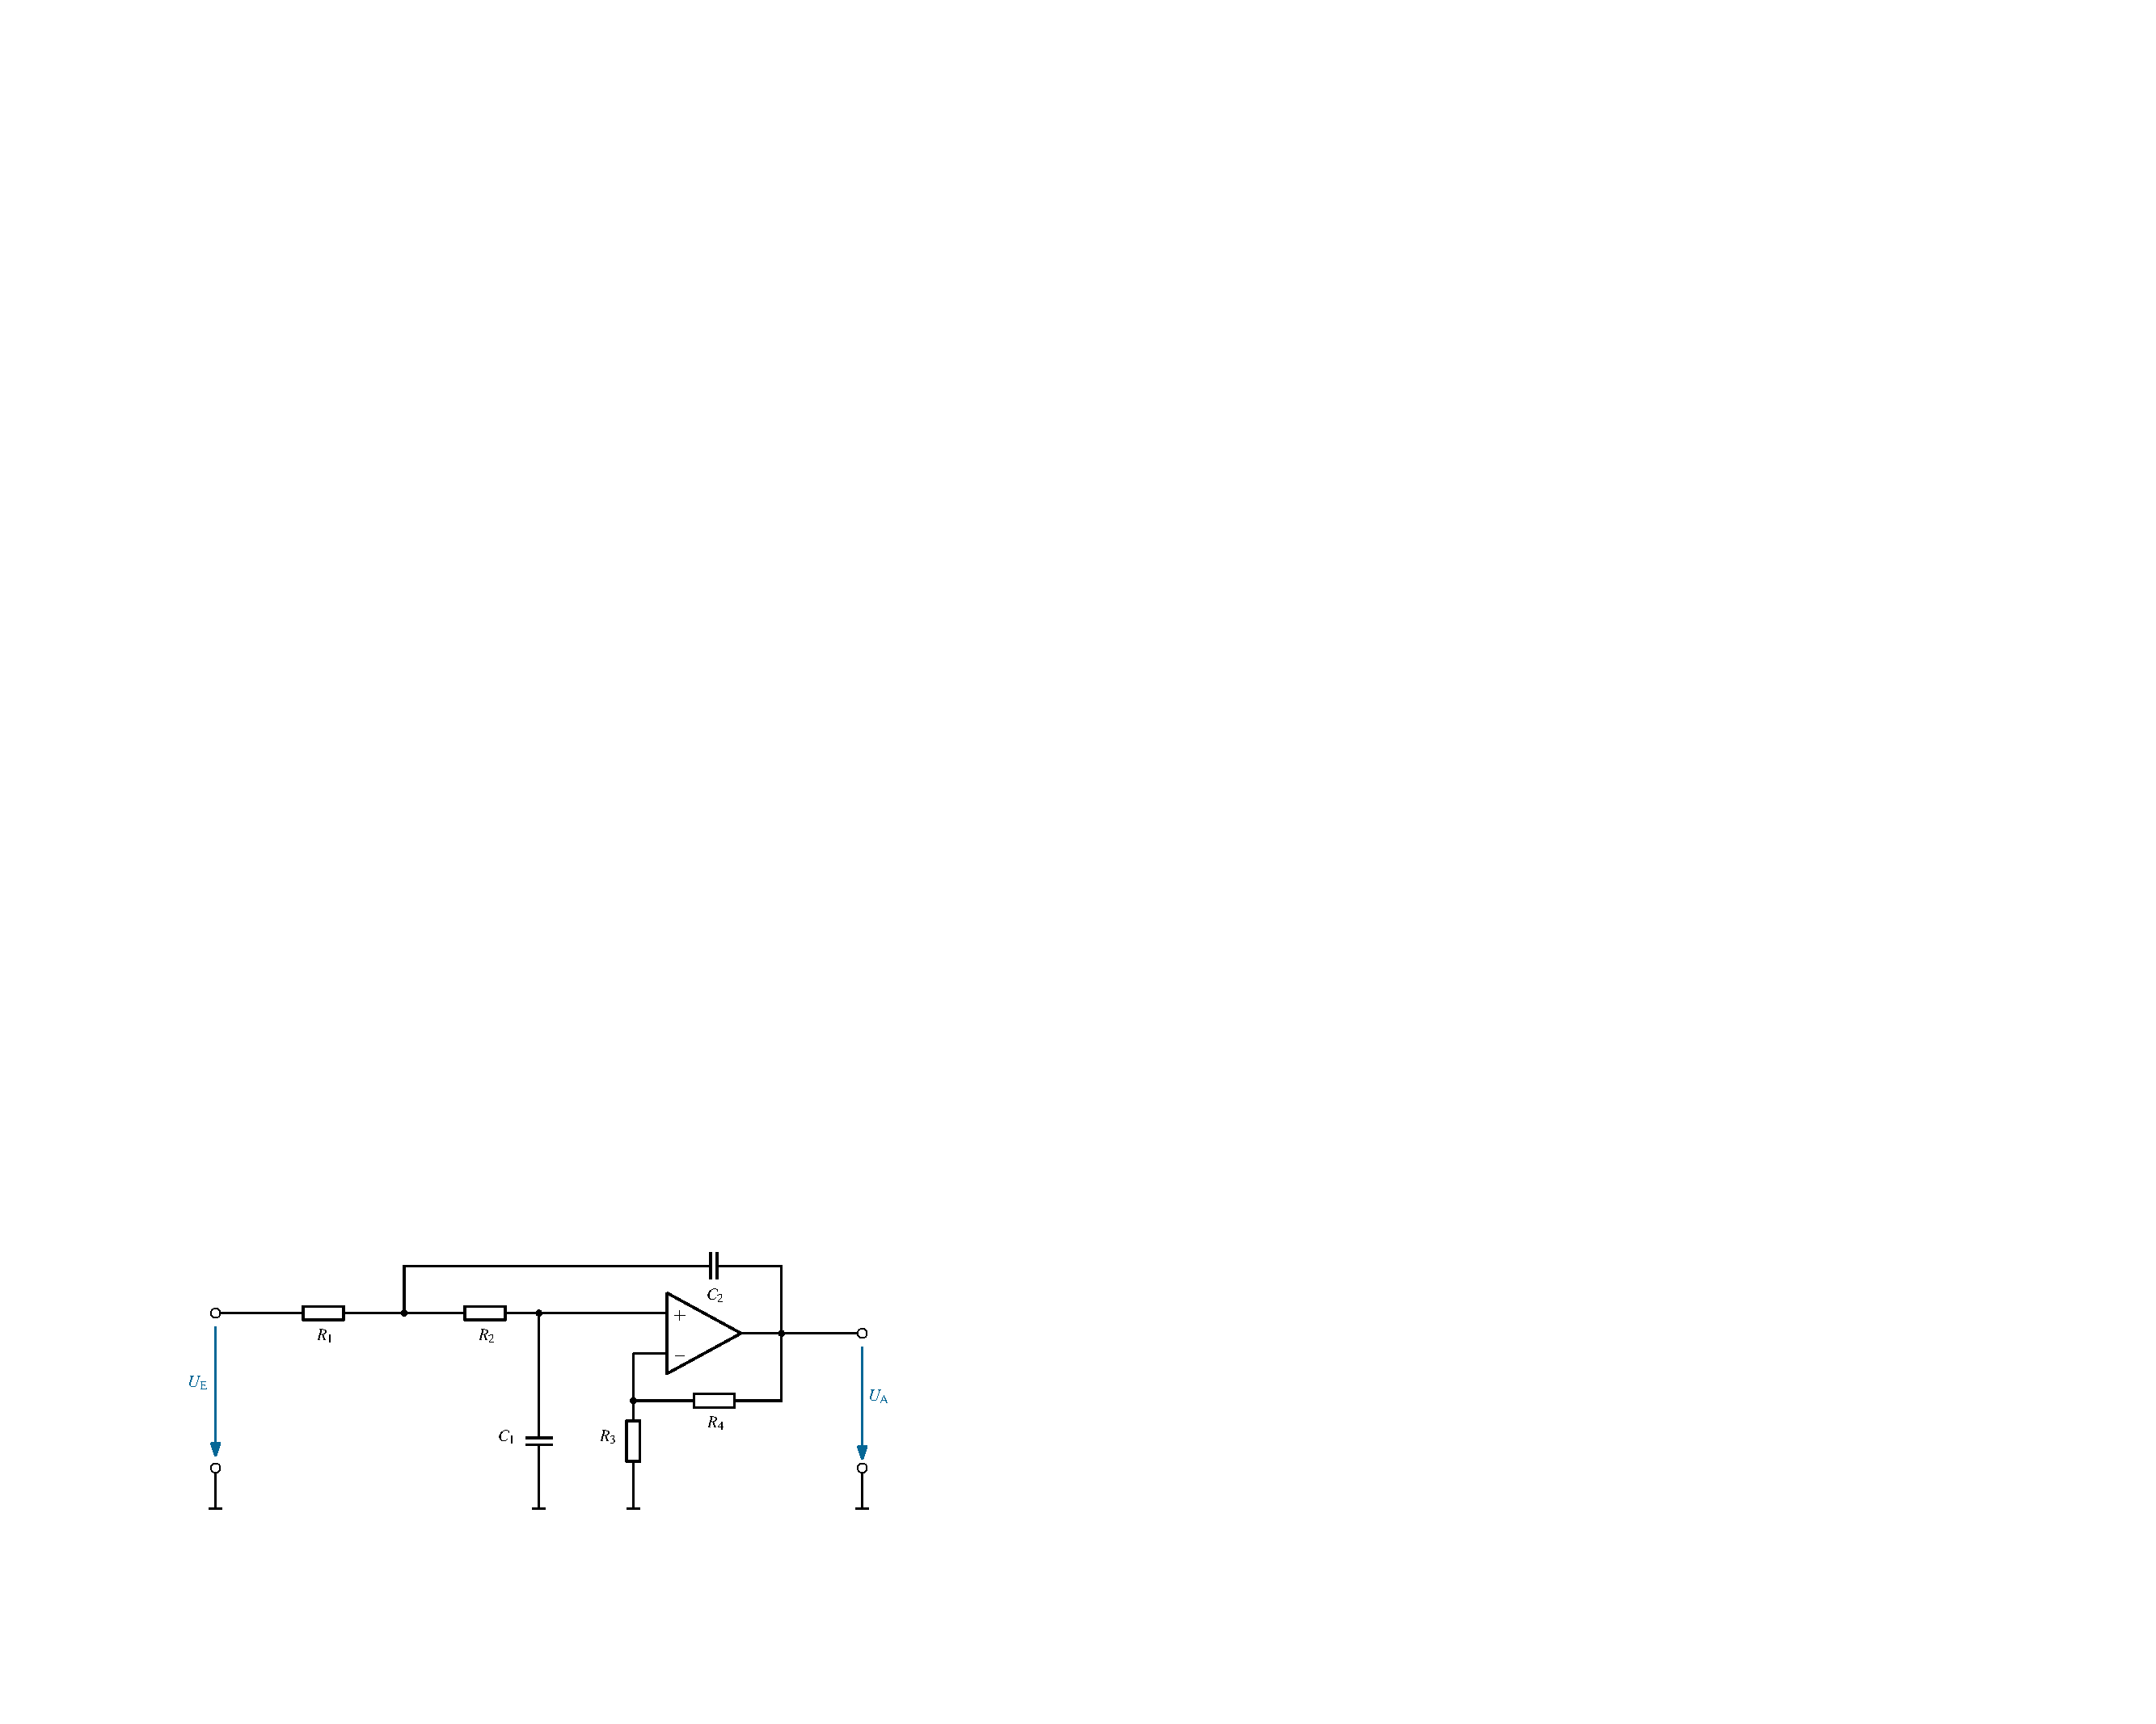
\includegraphics[scale=1]{schaltbild}|  erzugt ein
Bild an der Stelle des Aufrufes:

\begin{lstlisting}
  \begin{center}
    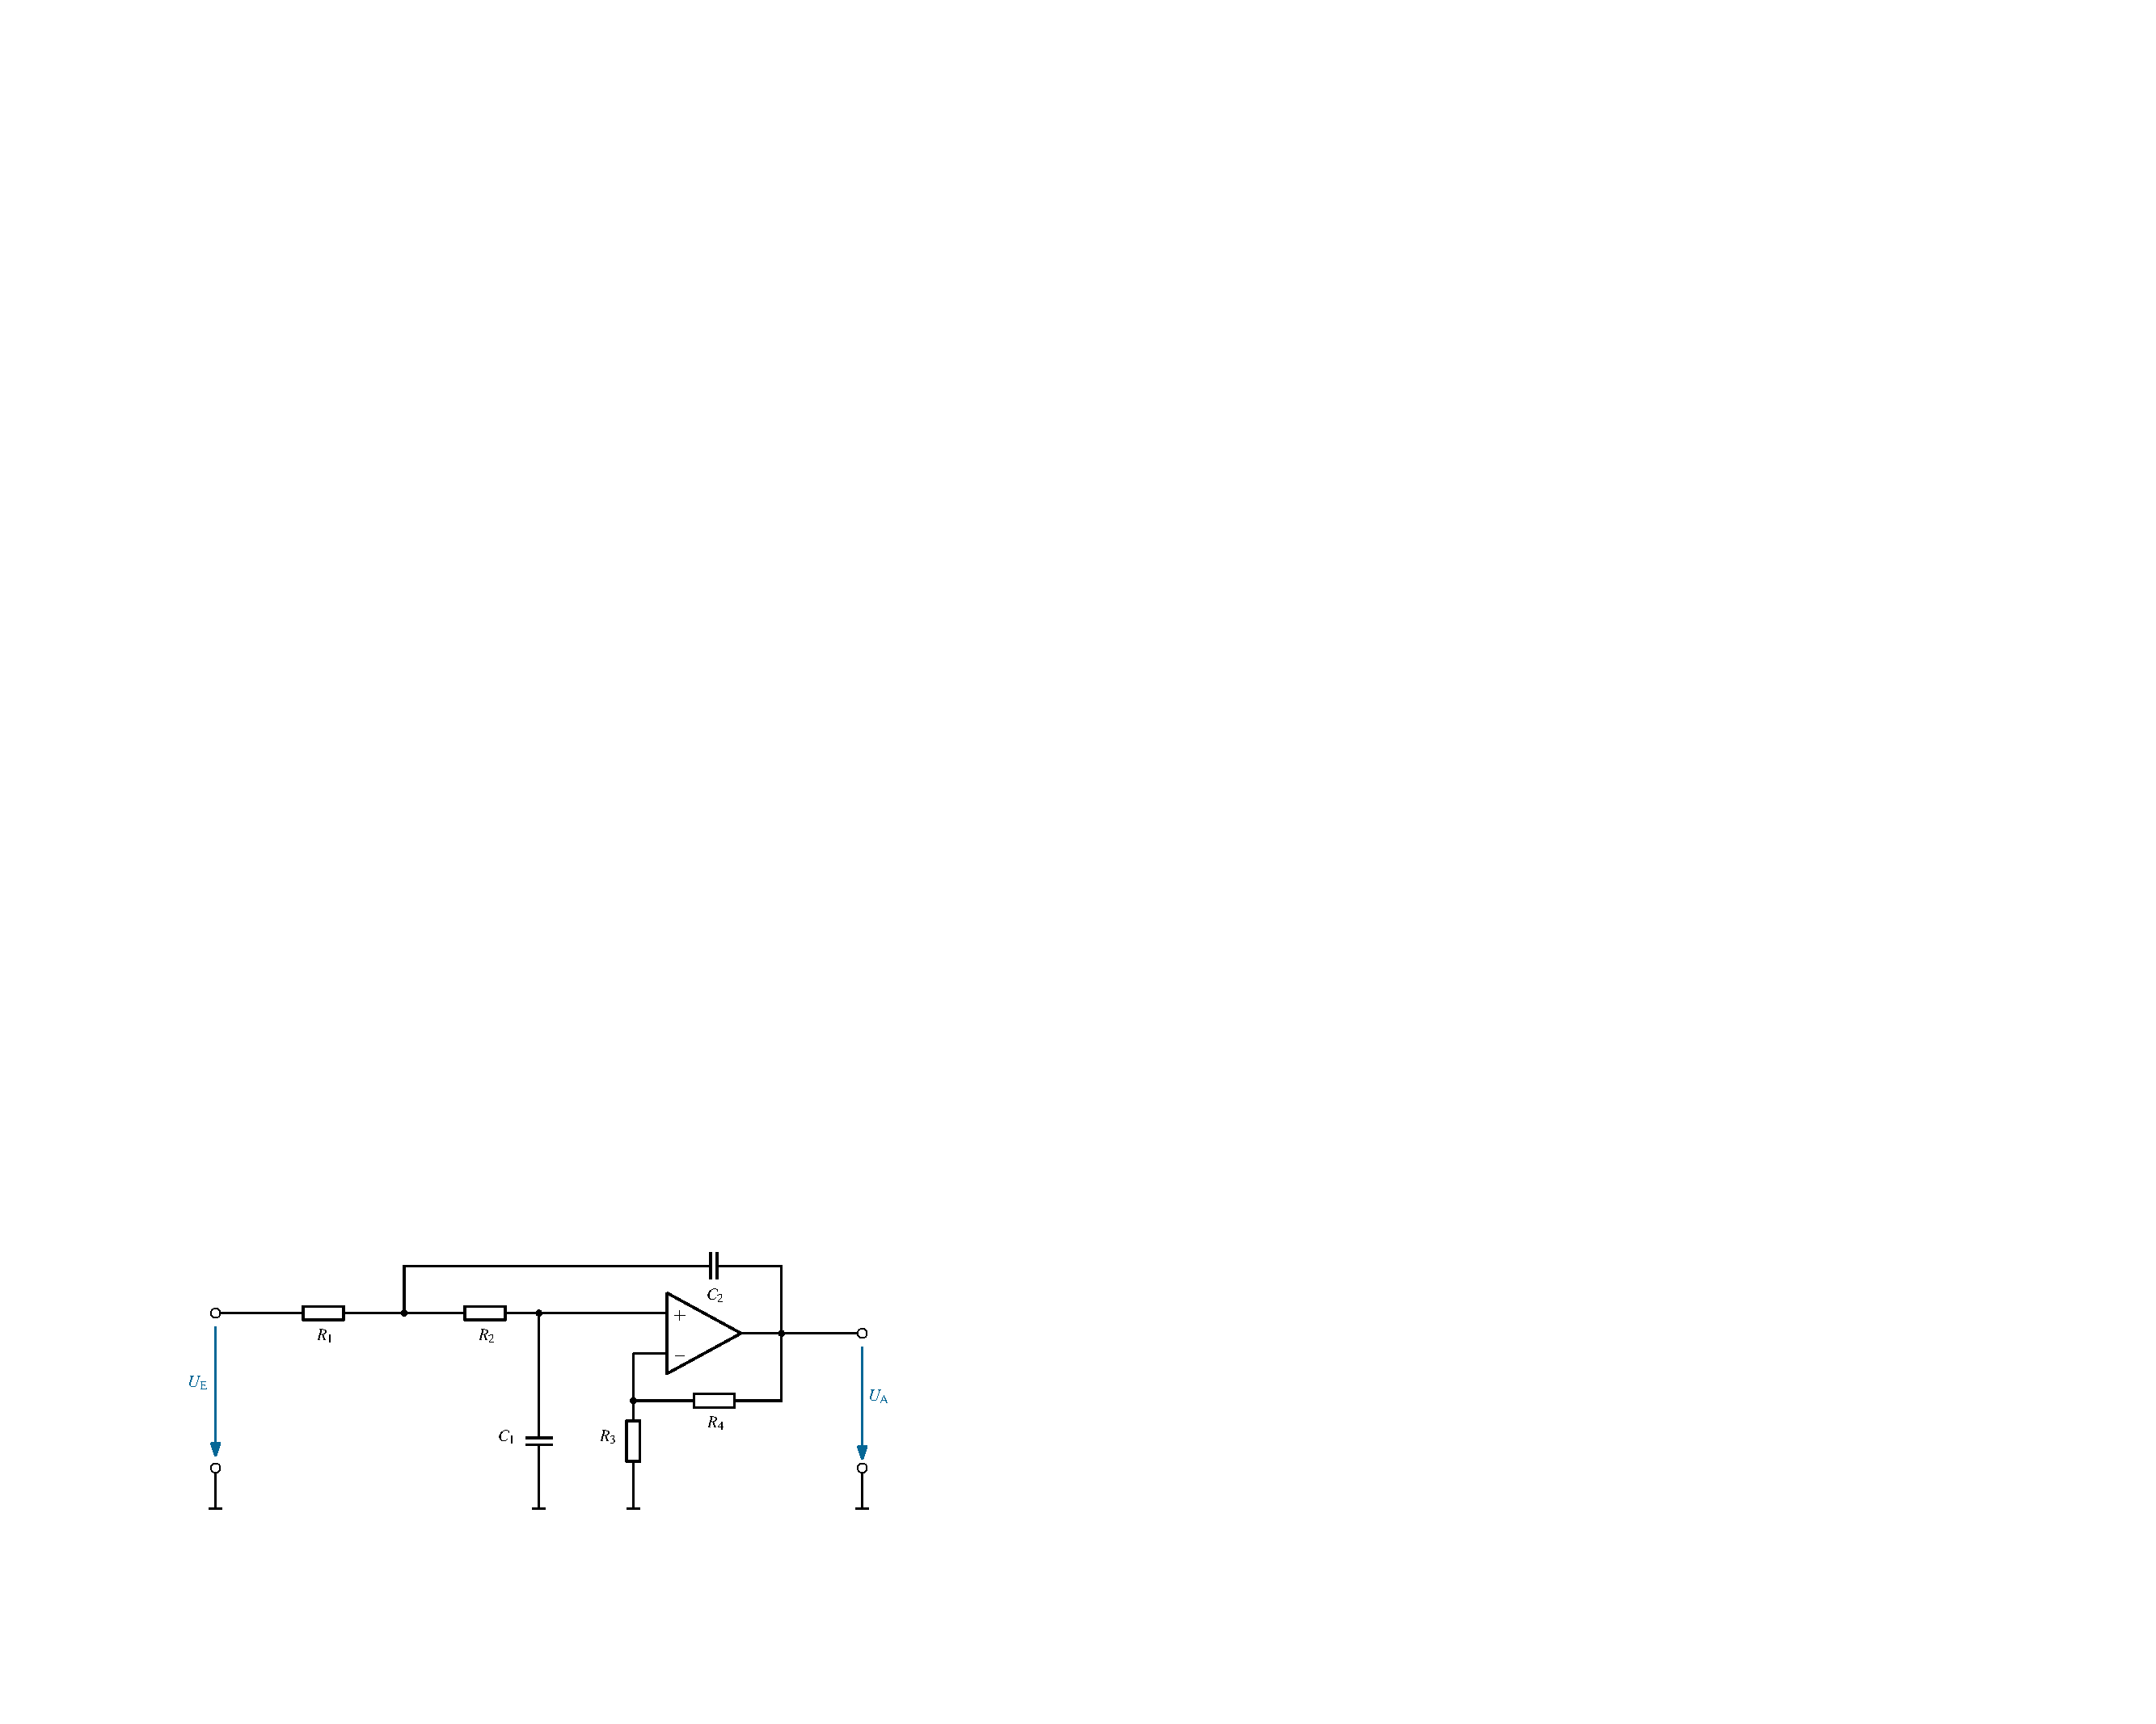
\includegraphics[scale=1]{schaltbild}
  \end{center}
\end{lstlisting}

\begin{center}
  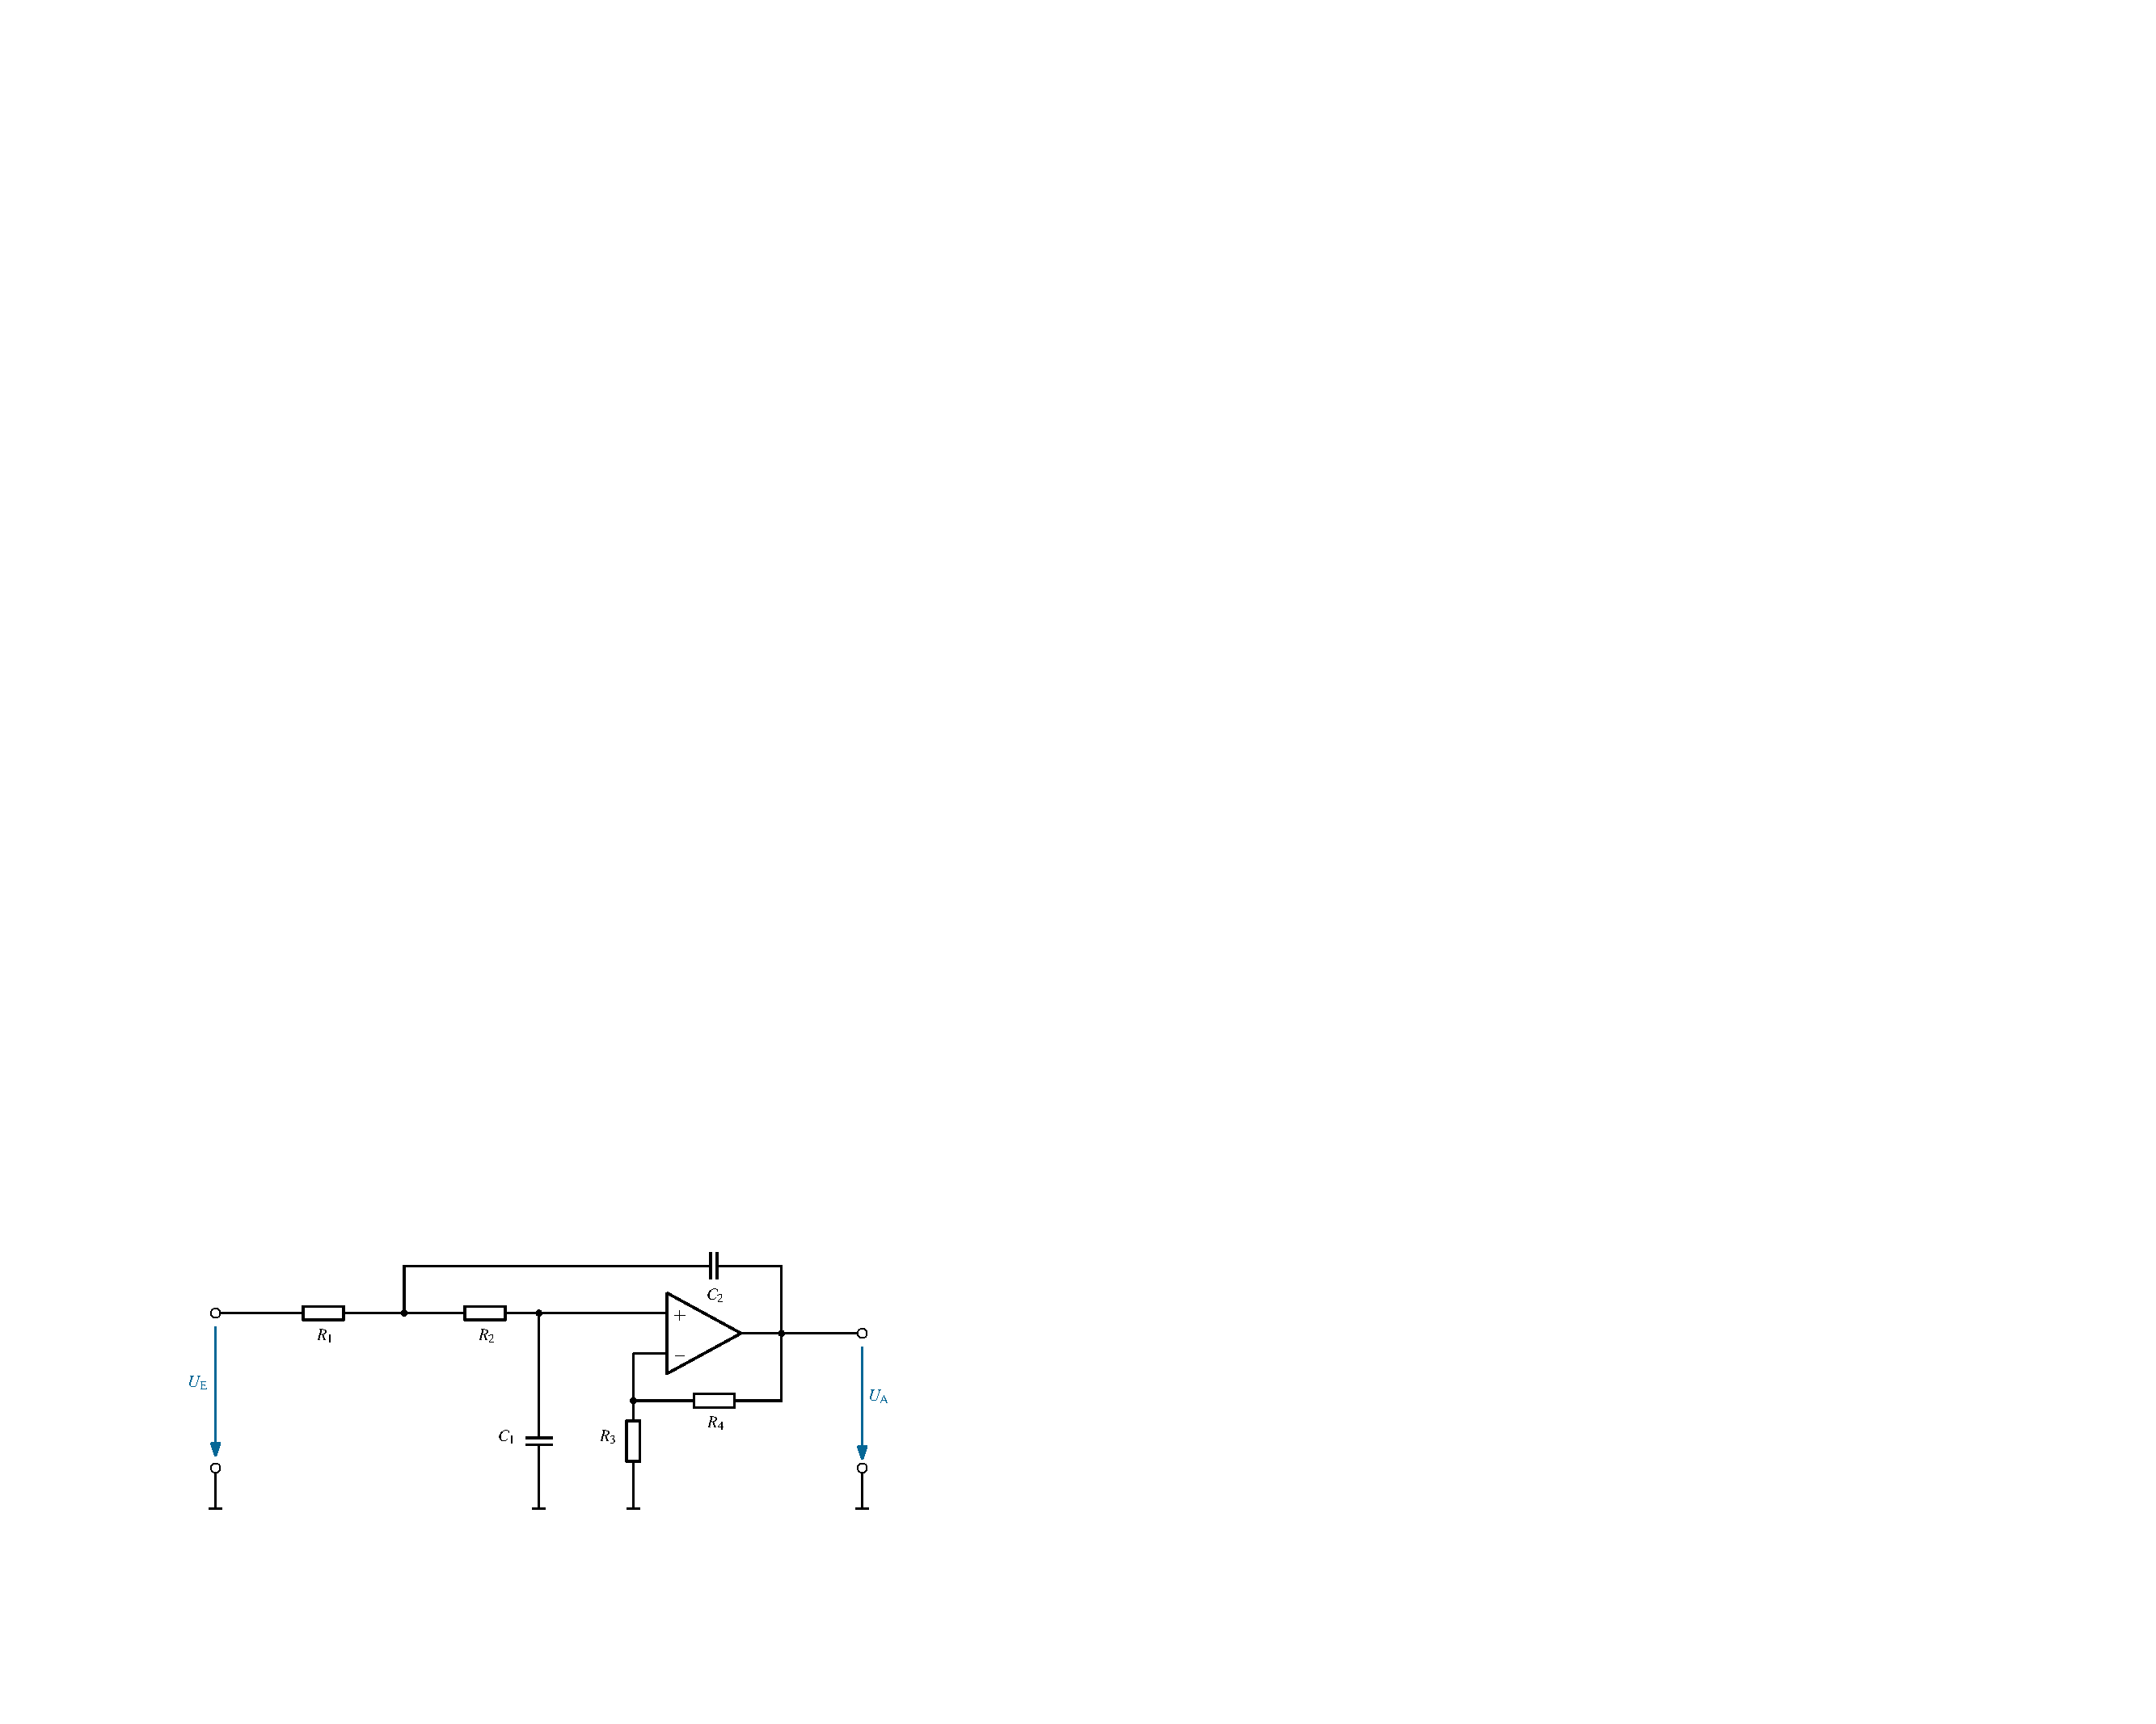
\includegraphics[scale=1]{schaltbild}
\end{center}

Es ist auch möglich, Abbildungen durch den Text \emph{fliessen} zu
lassen. \LaTeX\ kümmert sich um die Positionierung. Das Bild
\ref{fig.Filterschaltung} im Kapitel
\ref{ch.test} wird mit dem Folgenden code erzeugt:

\begin{lstlisting}
\begin{figure}[bht]
  \begin{center}
    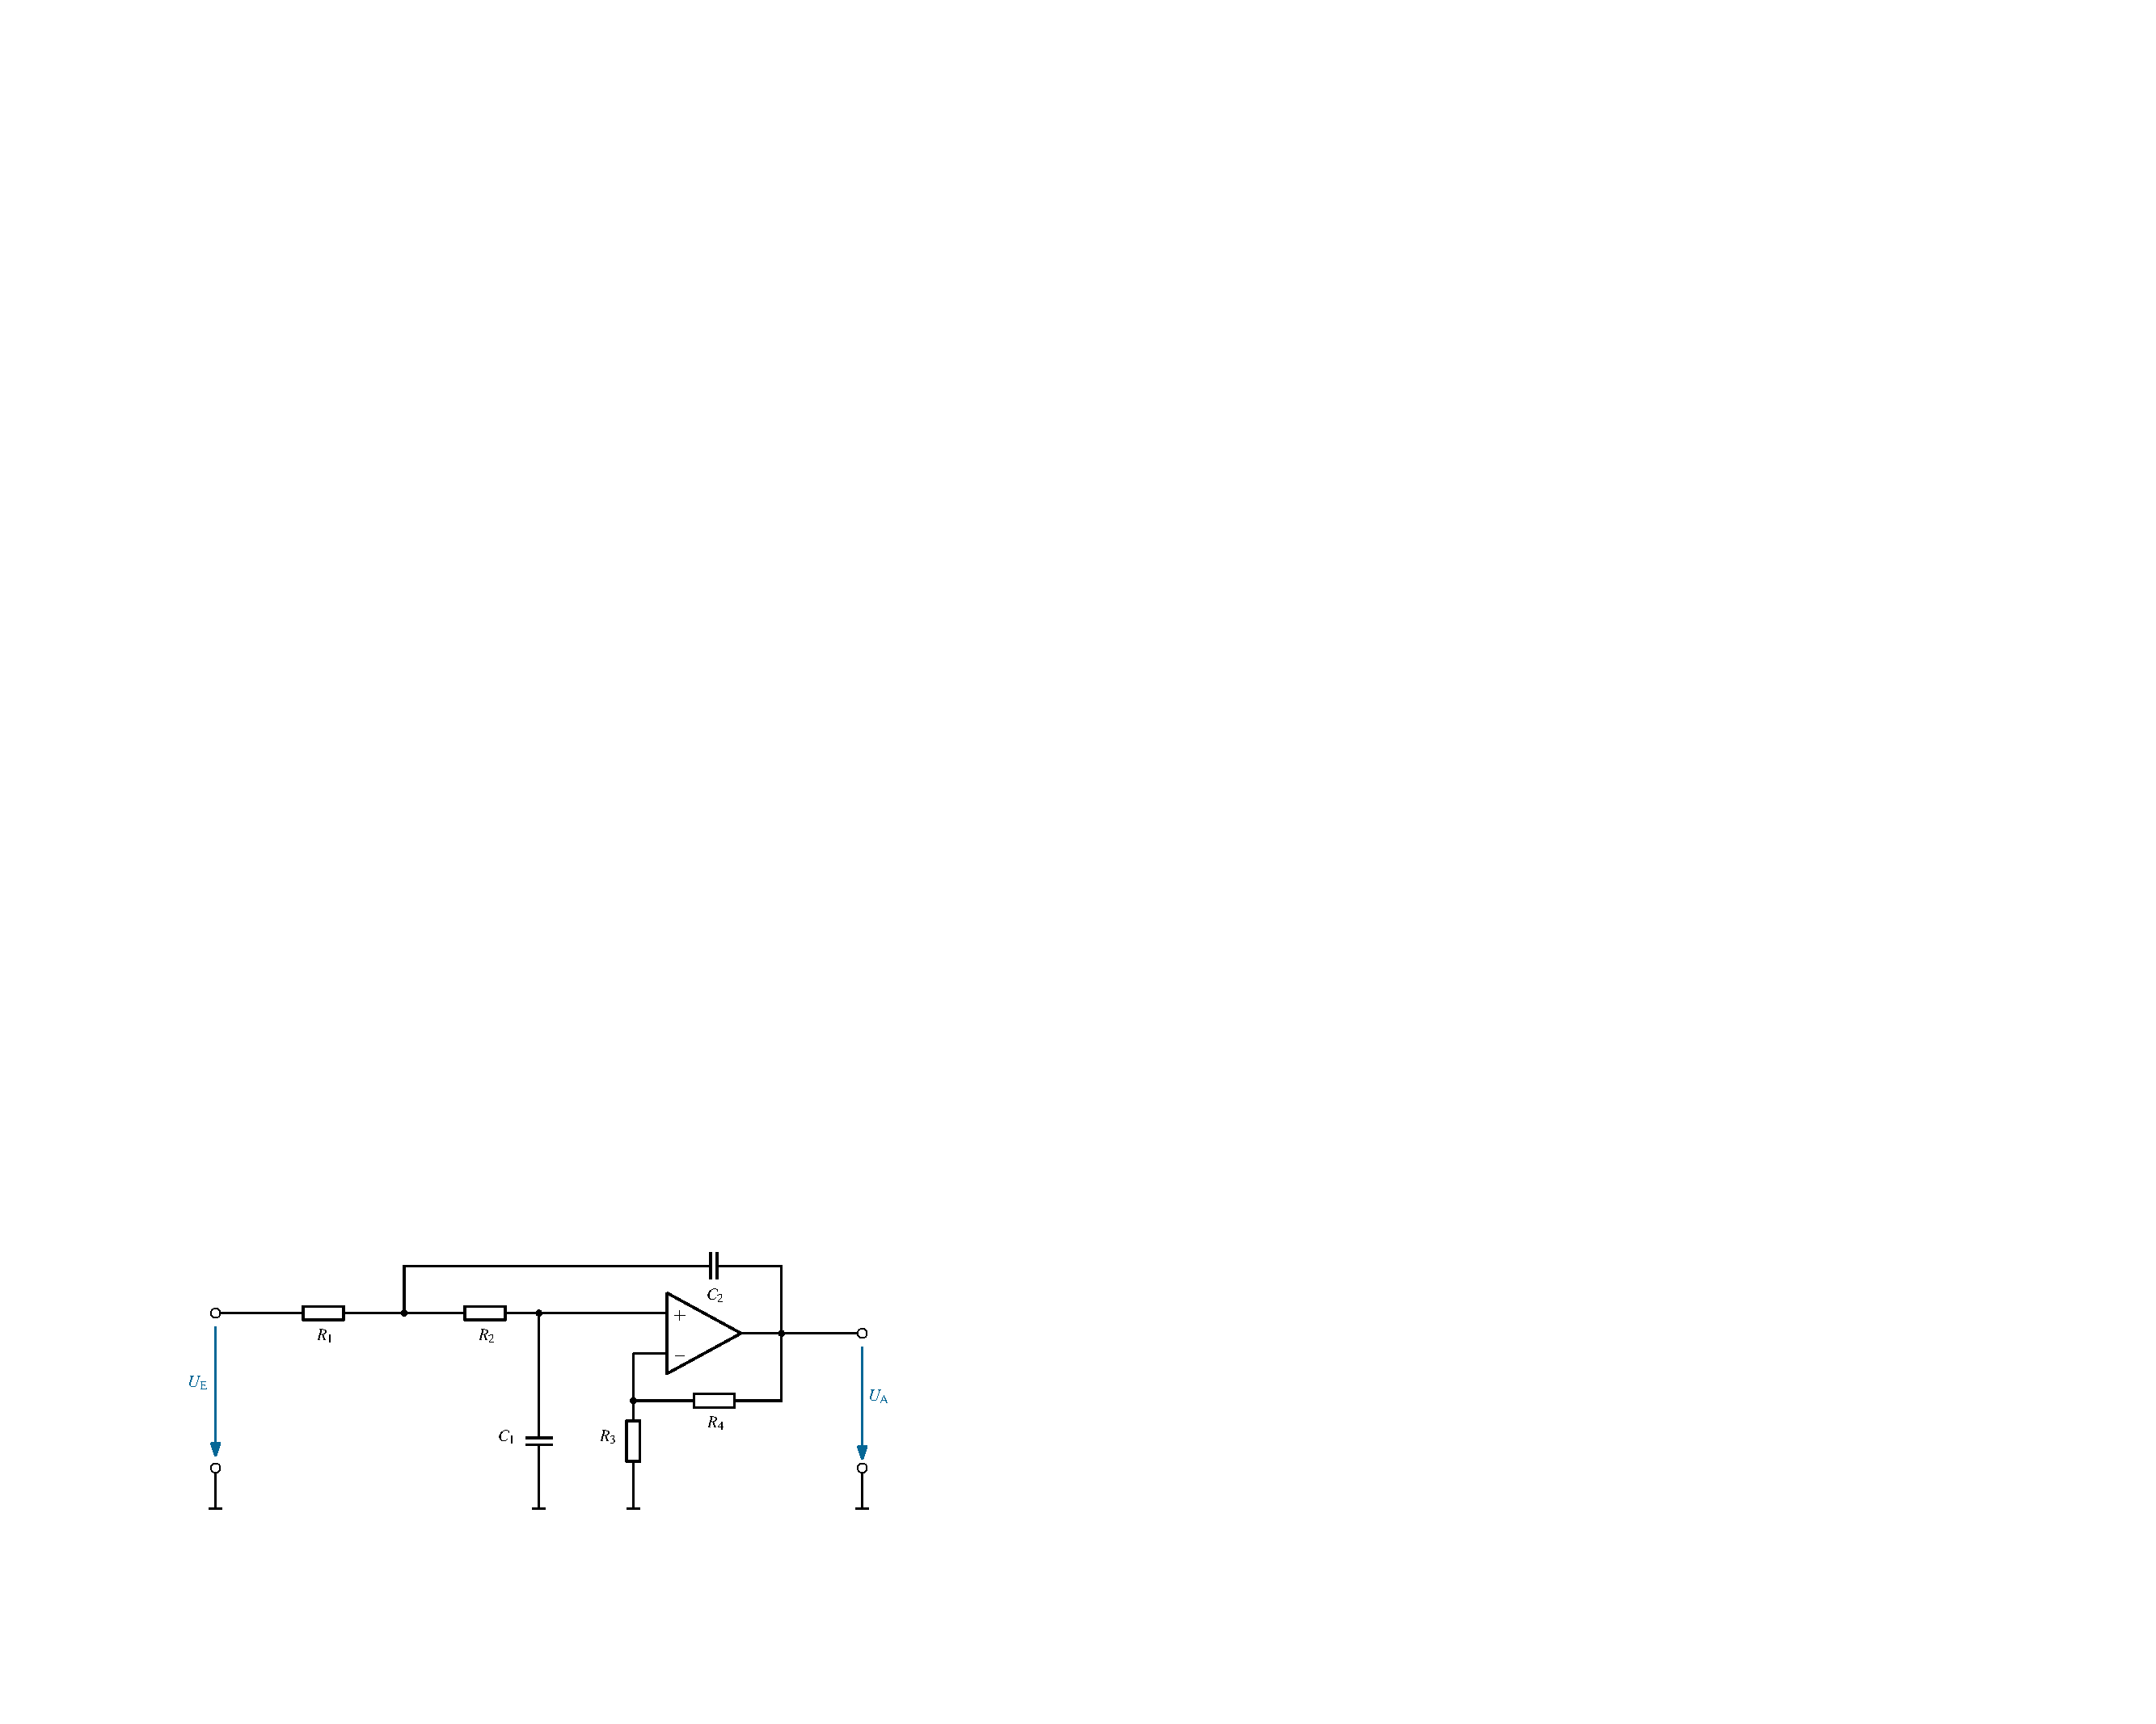
\includegraphics[scale=1]{schaltbild}
    \caption{Die verwendete Filterschaltung}
    \label{fig.Filterschaltung}
  \end{center}
\end{figure}
\end{lstlisting}

Hier ist zu  beachten, dass das Bild auch  automatisch in das Abbildungsverzeichnis
übernommen  wird.  Eine  Referenz  geschieht mit  \verb|\ref{fig.Filterschaltung}|.
Weiterhin braucht  \LaTeX\ etwas Text,  um Bilder darin \emph{fliessen}  zu lassen.
Jegliche Feinabstimmung sollte am Ende nach dem Schreiben des Textes passieren.


\section{Nützliches}

Der Textsatz kann durch viele Pakete in seiner Funktionalität erweitert
werden. Einige seien hier angeführt.

\paragraph{Transfomationssymbole}
Das Paket \texttt{trsym} definiert die Transformationssymbole fu Laplace- und
Fouriertransformation, wie Sie in einigen Lehrbüchern üblich sind.
\begin{equation}
  f(t)\,\TransformHoriz\,F(j\omega)
\end{equation} 
Viele   weitere  Symbole   und   deren  Möglichkeit   zur   Einbindung  werden   in
\cite{latex.symbols} beschrieben.

\paragraph{Querverweise anzeigen}
Das Paket \texttt{showkeys} zeigt alle  in Querverweisen verwendeten Marken im Text
an, so dass Fehler schneller gefunden werden können. 


%% \begin{bytefield}[boxformatting={\centering\itshape},
%%                   bitwidth=1.5em]{20}
%%   \bitheader[b]{0-19}   \\
%%   \bitbox{1}{\tiny F/E} & 
%%   \bitbox{1}{\tiny T0}  & 
%%   \bitbox{1}{\tiny T1}  & 
%%   \bitbox{1}{\tiny Fwd} & 
%%   \bitbox{16}{Data value} \\
%% \end{bytefield}

%%
%% Berliner Hochschule für Technik --  Abschlussarbeit
%%
%% Kapitel 2
%%
%%

\chapter{Zweiter Abschnitt}\label{ch.test}

In diesem Abschnitt folgt reichlich Blindtext, um das Aussehen voller Seiten zu
dokumentieren. 

\section{Grundlegendes}

\begin{neu}
  \blindtext \anno{Sachen gibt's!}
\end{neu}
\blindtext 

\section{Weiterführendes} 

\begin{neu}
  \blindtext
\end{neu}

\blindtext
\blindenumerate
\blindtext[3] \anno{Lesen, bitte!}

\begin{figure}[bht]
  \begin{center}
    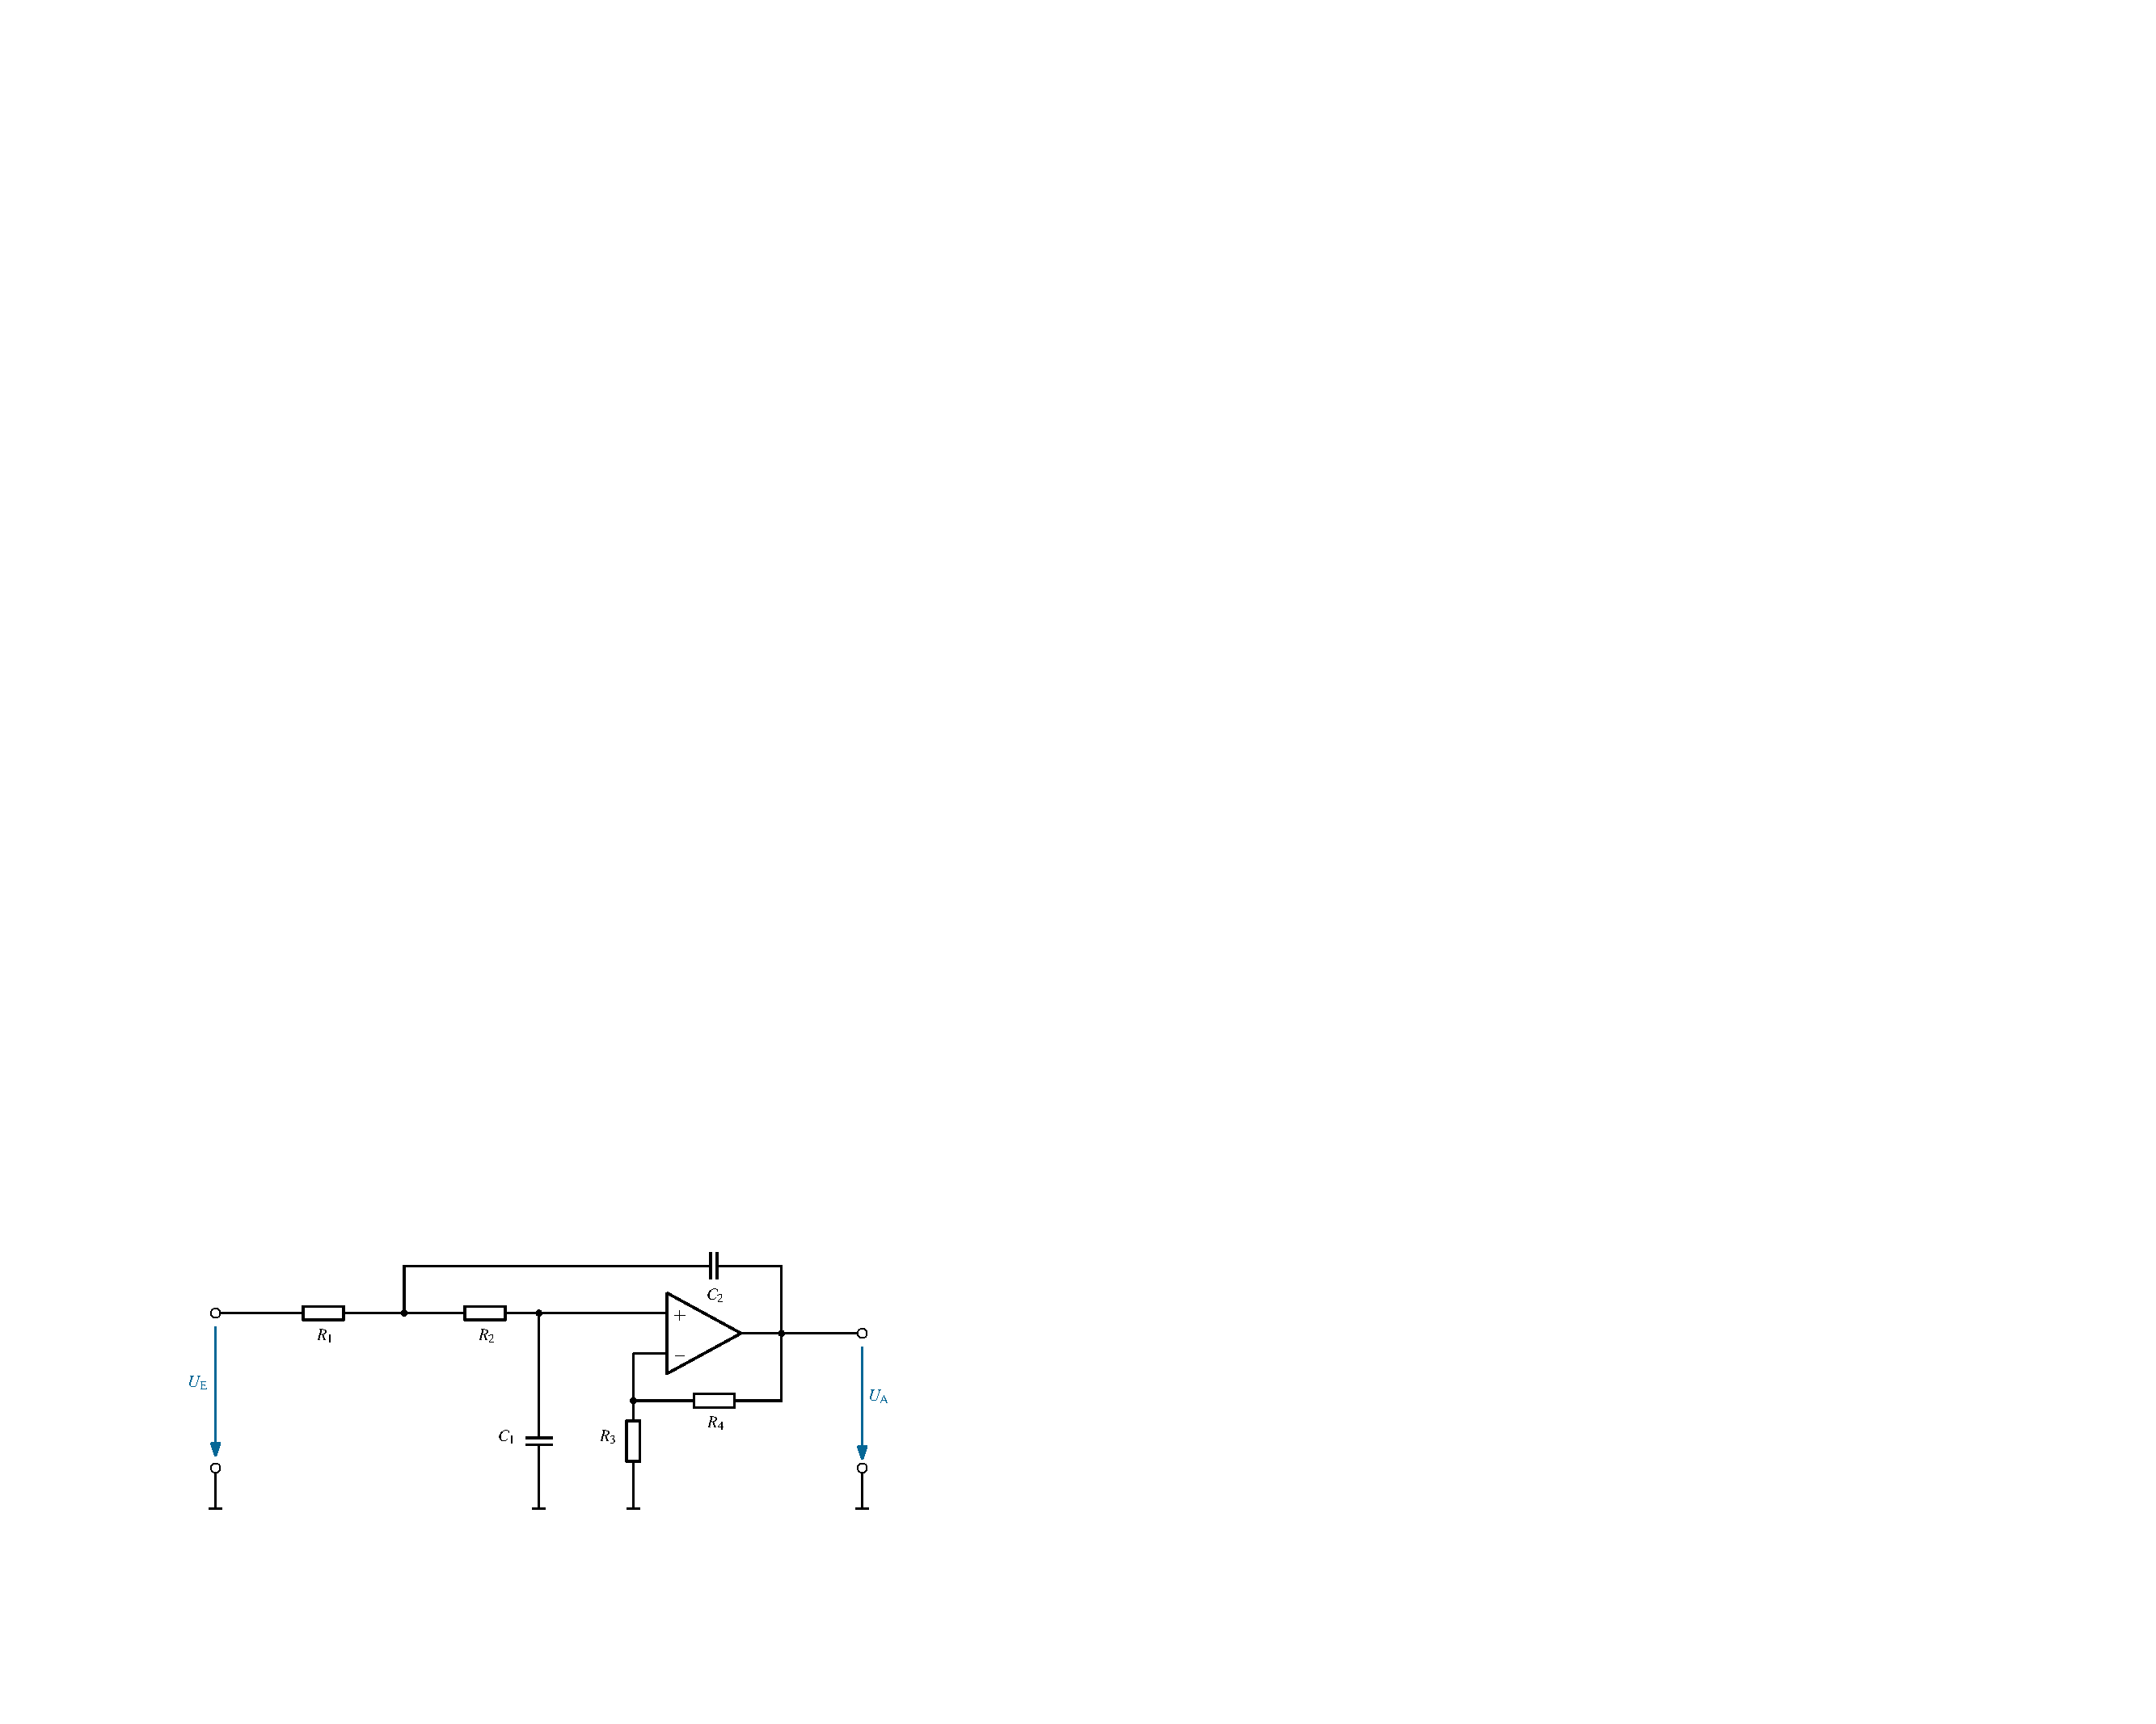
\includegraphics[scale=1]{schaltbild}
    \caption{Die verwendete Filterschaltung}
    \label{fig.Filterschaltung}
  \end{center}
\end{figure}

\blinditemize[8]
\Blindtext[2][2]
\blinddescription \anno{Es ist auch möglich längere Randnotizen zu machen. Ob die 
  dann aber gelesen werden, ist so eine Sache}  

\section{Abwegiges}

\blindtext



\begin{appendix}
  %%
%% Beuth Hochschule für Technik --  Abschlussarbeit
%%
%% Anhang
%%
%%%%%%%%%%%%%%%%%%%%%%%%%%%%%%%%%%%%%%%%%%%%%%%%%%%%%%%%%%%%%%%%%%%%%


\chapter{Angehängtes: Die Dateien des Pakets}

\subsection*{Tabellen}

\begin{table}[h]
  \centering
  \resizebox{\textwidth}{!}{
    \begin{tabular}{|c | c | c | c |} 
 \hline
      \textbf{WAF Name} & \textbf{Hersteller} & \textbf{WAF Name} & \textbf{Hersteller} \\
      \hline
      ACE XML Gateway & Cisco & FirePass & F5 Networks\\
      Airlock & Phion/Ergon & FortiWeb & Fortinet\\
      Alert Logic & Alert Logic & GoDaddy Website Protection & GoDaddy\\
      AliYunDun & Alibaba Cloud Computing & Huawei Cloud Firewall & Huawei\\
      AnYu & AnYu Technologies & HyperGuard & Art of Defense\\
      AppWall & Radware & Imunify360 & CloudLinux\\
      Armor Defense & Armor & Incapsula & Imperva Inc.\\
      ArvanCloud & ArvanCloud & ISA Server & Microsoft\\
      ASP.NET Generic & Microsoft & Janusec Application Gateway & Janusec\\
      ASPA Firewall & ASPA Engineering Co. & Kona SiteDefender & Akamai\\
      Astra & Czar Securities & KS-WAF & KnownSec\\
      AWS Elastic Load Balancer & Amazon & LimeLight CDN & LimeLight\\
      AzionCDN & AzionCDN & Oracle Cloud & Oracle\\
      Azure Front Door & Microsoft & ModSecurity & SpiderLabs\\
      Barracuda & Barracuda Networks & NetContinuum & Barracuda Networks\\
      Bekchy & Faydata Technologies Inc. & NetScaler AppFirewall & Citrix Systems\\
      Beluga CDN & Beluga & NullDDoS Protection & NullDDoS\\
      BinarySec & BinarySec & PentaWAF  & Global Network Services\\
      BitNinja & BitNinja &   PT Application Firewall & Positive Technologies\\
      BlockDoS & BlockDoS &   Profense  & ArmorLogic\\
      Bluedon & Bluedon IST &   Qcloud   & Tencent Cloud\\
      CacheWall & Varnish &   RequestValidationMode   & Microsoft\\
      CacheFly CDN & CacheFly &   Sabre Firewall     & Sabre\\
      Comodo cWatch & Comodo CyberSecurity &   eEye SecureIIS & BeyondTrust\\
      CdnNS Application Gateway & CdnNs/WdidcNet &   SecuPress WP Security  & SecuPress\\
      ChinaCache Load Balancer & ChinaCache &   SecureSphere  & Imperva Inc.\\
      Chuang Yu Shield & Yunaq &   SEnginx       & Neusoft\\
      Cloudbric & Penta Security &   SiteGuard  & Sakura Inc.\\
      Cloudflare & Cloudflare Inc. &   SonicWall   & Dell\\
      Cloudfloor & Cloudfloor DNS &   UTM Web Protection              & Sophos\\
      Cloudfront & Amazon &   SquidProxy IDS   & SquidProxy\\
      CrawlProtect & Jean-Denis Brun &   Tencent Cloud Firewall   & Tencent Technologies\\
      DataPower & IBM &   Teros   & Citrix Systems\\
      DenyALL & Rohde+Schwarz CyberSecurity &  Trafficshield  & F5 Networks\\
      Distil & Distil Networks &   Varnish        & OWASP\\
      DotDefender & Applicure Technologies &   WebSEAL  & IBM\\
      DynamicWeb Injection Check & DynamicWeb &   XLabs Security WAF   & XLabs\\
      BIG-IP AppSec Manager & F5 Networks &   ZScaler & Accenture\\
      BIG-IP AP Manager & F5 Networks & & \\
      Fastly & Fastly & & \\
      \hline
      
      
\end{tabular}}
\caption{Auszug WAFw00f Plugins(aus https://github.com/EnableSecurity/wafw00f)}
\medskip
\small
WAFw00f ist ein Werkzeug zur Identifikation von WAFs und die Liste der Plugins gleichzeitig eine Liste der WAF-Produkte die WAFw00f erkennt.
\label{tab:my_wafwoof}
\end{table}

\begin{table}[h]
  \centering
%  \resizebox{\textwidth}{!}{
  \begin{tabular}{|l | p{7cm} |}
    \hline
    \textbf{Name} & \textbf{Beschreibung} \\
    \hline
    gotestwaf & tool for API and OWASP attack simulation \\
    BurpSuite & vulnerability scanning, penetration testing, and web app security platform\\
    identYwaf & identification tool that can recognize web protection \\
    lightbulb-framework & framework for auditing web application firewalls \\
    OWASP Zed Attack Proxy & the world's most widely used web app scanner \\
    Paros Proxy & A Java based HTTP/HTTPS proxy for assessing web application vulnerability.\\
    sqlmap & testing tool that automates SQL injection\\
    w3af & Web Application Attack and Audit Framework\\
    weka & Waikato Environment for Knowledge Analysis - collection of ML algorithms for data mining tasks\\
    waf-brain & WAF - the Machine-Learning-Deep-Learning-Way\\
    waf-bypass & open source tool to analyze the security of an WAF\\
    WAFNinja &  WAFNinja is a tool which contains two functions to attack Web Application Firewalls. \\
    wafw00f & allows one to identify and fingerprint Web Application Firewall products\\
    \hline
    % \end{tabular}}    
  \end{tabular}
  
  \caption{Übersicht Werkzeuge}
  \medskip
  \small
  (Die Beschreibung der Werkzeuge wurde den jeweiligen Internetpräsenzen entnommen)
  \label{tab:my_tools}
\end{table}

\begin{table}[h]
  \centering
  \begin{tabular}{|l|}
    \hline
    Eclipse CargoTracker \\
    J2EE PetStore \\
    Spring PetClinic \\
    JBoss QuickStarts (KitchenSink) \\
    PrimeFaces Showcase \\
    \hline
  \end{tabular}
  \caption{Übersicht Demo Anwendungen}
  \label{tab:exampleapp}
\end{table}

\begin{table}[h]
  \centering
  \begin{tabular}{|l|}
    \hline
    JavaVulnerableLab \\
    Marathon\\
    VulnarableSpring \\
    OWASP Mutillidae II \\
    OWASP WebGoat \\
    \hline
  \end{tabular}
  \caption{Übersicht Absichtlich angreifbare Anwendungen}
  \label{tab:vulnapp}
\end{table}

\begin{table}[h]
  \centering
  \begin{tabular}{|l|}
    \hline
    \textbf{Feature Name} \\
    \hline
    Length of the request \\
    Length of the path \\
    Length of the arguments \\
    Length of the header \glqq\emph{Accept}\grqq \\
    Length of the header \glqq\emph{Accept-Encoding}\grqq \\
    Length of the header \glqq\emph{Accept-Charset}\grqq \\
    Length of the header \glqq\emph{Accept-Language}\grqq \\
    Length of the header \glqq\emph{Cookie}\grqq \\
    Length of the header \glqq\emph{Content-Length}\grqq \\
    Length of the header \glqq\emph{Content-Type}\grqq \\
    Length of the Host \\
    Length of the header \glqq\emph{Referer}\grqq \\
    Length of the header \glqq\emph{User-Agent}\grqq \\
    Method identifier\\
    Number of arguments\\
    Number of letters in the arguments\\
    Number of digits in the arguments\\
    Number of special char in the arguments\\
    Number of other char in the arguments\\
    Number of letters in the path\\
    Number of digits in the path\\
    Number of special char in the path\\
    Number of other char in the path\\
    Number of cookies\\
    Minimum byte value in the request\\
    Maximum byte value in the request\\
    Number of distinct bytes\\
    Entropy\\
    Number of keywords in the path\\
    Number of keywords in the arguments\\
    \hline
  \end{tabular}
  \caption{Names of 30 expert knowledge features that are considered relevant for the detection of web attacks for the CSIC dataset (s. Tabelle 5.2. in \cite{Giménez2015})}
  \label{tab:tgfeatures}
\end{table}

\end{appendix}
%%%%%%%%%%%%%%%%%%%%%%%%%%%%%%%%%%%%%%%%%%%%%%%%%%%%%%%%%%%%%%%
%% Literaturverzeichnis

\clearpage\newpage
\addcontentsline{toc}{chapter}{Literatur- und Quellenverzeichnis}
\bibliographystyle{myapalike}
\bibliography{bhtThesis}

\end{document}
